%%% template.tex
%%%
%%% This LaTeX source document can be used as the basis for your technical
%%% paper or abstract.
%%%
%%% This example is tailored toward the two-page abstract. Please see "template.tex"
%%% for a more fully-annotated example.

\documentclass[final]{acmsiggraph}

\let\bibhang\undefined % delete the definition from acmsiggraph.cls
\usepackage{natbib} 
\setlength{\bibhang}{1em}
\bibpunct{[}{]}{;}{a}{}{,}
\bibliographystyle{tognat} % use with natbib

\usepackage{microtype}
\usepackage{amsmath}
\renewcommand{\ttdefault}{cmtt}

% for complicated tables
\usepackage{tabularx, booktabs}
\usepackage{multirow}
\usepackage[table]{xcolor}
\usepackage{dcolumn}

%%% Title of your article or abstract.

\title{Triangle Reordering for Reduced Overdraw in Animated Scenes}

\author{ Songfang Han$\qquad$Pedro V. Sander\\[3pt]
  Hong Kong UST}
\pdfauthor{Songfang Han and Pedro V. Sander}

%%% Used by the ``review'' variation; the online ID will be printed on 
%%% every page of the content.

\TOGonlineid{129}

% User-generated keywords.

\keywords{real-time rendering, depth sorting, overdraw reduction}


%\newcommand{\citep}[1]{\cite{#1}}
\newcommand{\remark}[1]{\textcolor{red}{#1}}
\newcommand{\reremark}[1]{\textcolor{blue}{#1}}
\newcommand{\ignore}[1]{}

% With the "\setcopyright" command the appropriate rights management text will be added
% to your document.

%\setcopyright{none}
\setcopyright{acmcopyright}
%\setcopyright{acmlicensed}
%\setcopyright{rightsretained}
%\setcopyright{usgov}
%\setcopyright{usgovmixed}
%\setcopyright{cagov}
%\setcopyright{cagovmixed}
%\setcopyright{rightsretained}

% The year of publication in the "\copyrightyear" command.

\copyrightyear{2016}

%%% Conference information, from the completed rights management form.
%%% The "\conferenceinfo" command has two parameters: 
%%%    - conference name
%%%    - conference date and location
%%% The "\isbn" field includes the year and month after the article ISBN.

\conferenceinfo{I3D '16, ACM SIGGRAPH Symposium on
Interactive 3D Graphics and Games}{February 27-28, Redmond, WA, USA.}
\isbn{978-1-4503-4043-4/16/03 \$15.00}
\doi{http://dx.doi.org/10.1145/2856400.2856408}

\begin{document}

%%% This is the ``teaser'' command, which puts an figure, centered, below 
%%% the title and author information, and above the body of the content.

 \teaser{
{\hfill\includegraphics[width=\textwidth]{images/teaser}\hfill}
\caption{Renderings of the four animated characters used in our results. The small images visualize overdraw for several key frames in the animation (dark regions indicate overdraw). Refer to the supplemental video for a full demonstration.}
\label{fig:teaser}
\vspace*{-4pt}
 }

\maketitle

\begin{abstract}

We introduce an automatic approach for optimizing the triangle rendering order of animated
meshes with the objective of reducing overdraw while maintaining good post-transform vertex
cache efficiency. Our approach is based on prior methods designed for static meshes. We propose
an algorithm that clusters the space of viewpoints and key frames. For each
cluster, we generate a triangle order that exhibits satisfactory vertex cache efficiency and low overdraw. Results 
show that our approach significantly improves overdraw throughout the entire animation sequence while only 
requiring a few index buffers. We expect that this approach will be useful for games and other real-time
rendering applications that involve complex shading of articulated characters.

\end{abstract}

%
% The code below should be generated by the tool at
% http://dl.acm.org/ccs.cfm
% Please copy and paste the code instead of the example below. 
%
\begin{CCSXML}
<ccs2012>
<concept>
<concept_id>10010147.10010371.10010372.10010377</concept_id>
<concept_desc>Computing methodologies~Visibility</concept_desc>
<concept_significance>500</concept_significance>
</concept>
</ccs2012>
\end{CCSXML}

\ccsdesc[500]{Computing methodologies~Visibility}

%
% End generated code
%

% The next three commands are required, and insert the user-generated keywords, 
% The CCS concepts list, and the rights management text.
% Please make sure there is a blank line between each of these three commands.

\keywordlist

\conceptlist

\printcopyright

\setlength{\parskip}{5pt plus 1pt minus 1pt}
\section{Introduction}

Advanced real-time rendering applications often involve rendering large animated models using complex lighting and shading techniques. Depending of the relative complexity between the rendered geometry and the fragment shading algorithm, the rendering process is often bottlenecked at either the {\em vertex shader} or {\em fragment shader} stage. Scenes that fall into one of these categories are referred to as  {\em vertex-bound} and {\em fill-bound} scenes, respectively. Approaches have been proposed to reorder the triangles of a mesh so as to alleviate these bottlenecks.

In order to reduce vertex computation, the application can leverage the GPU's post-transform vertex caching mechanism, which stores the vertex shading output of a small set of recently processed vertices. When processing a particular vertex, recomputation can be avoided if the vertex has recently been processed by an adjacent triangle within the same hardware unit and thus is still cached. This encourages a triangle order with vertex reference locality (i.e., mesh triangles that share vertices should be close to each other in the index buffer). The average cache miss ratio (ACMR) of a particular triangle order measures the ratio between processed vertices and rendered triangles for a given caching scheme (usually a FIFO scheme is assumed). Generating triangle orders that reduce ACMR results in a significant improvement in rendering time for heavily vertex-bound scenes.

Scenes may also have very complex lighting and shading techniques, resulting in computationally intensive fragment shaders. In this case, reducing the number of fragments that need to be shaded can significantly reduce rendering time. When rasterizing triangles, GPUs apply {\em early-Z culling}, which performs depth testing prior to fragment shading. Thus, if the triangles happen to be processed in perfect front-to-back order, {\em none} of the occluded fragments will need to be shaded. In the worst case, when rendering in back-to-front order, {\em all} of the fragments need to be shaded, even those that are completely occluded by subsequent triangles. The overdraw ratio (OVR) of a triangle order refers to the ratio between the total number of fragments that passed the depth test and the number of visible fragments. An overdraw ratio of 1 is optimal and means no overdraw.

It has been shown that for heavily vertex-bound scenes, ACMR is directly proportional to rendering time, while for heavily fill-bound scenes, OVR is directly proportional to rendering time~\citep{Sander07}. An efficient triangle order has both low ACMR and low OVR. In this paper we propose a technique that, as in \cite{Nehab06} and \cite{Sander07}, compromises between these two objectives. However, unlike these previous techniques, our approach handles animated meshes. Since we are addressing keyframe animations where mesh connectivity does not change, ACMR is invariant to the animation. On the other hand, since vertices change their relative positions over the course of the animation, OVR can be significantly affected. Our algorithm generates a set of triangle orders that minimize OVR over the entire animation sequence, while still maintaining a low ACMR.
\section{Related work}
\label{sec:prevwork}

\paragraph{Vertex caching}
Vertex cache optimization has been extensively researched.
Early techniques made advances by reducing bandwidth and generating compressed data structures, such as triangle strips (e.g., ~\cite{Akeley90, Deering95, Chow97}).
More recent methods simply utilize the transparent caching provided by modern GPUs and just reorder the triangles without
further compressing the index buffer (e.g.,~\cite{Hoppe99, Lin06, Sander07}). These approaches directly target the post-transform cache, where most of the vertex
processing gain can be achieved. In this paper, we do not propose new methods for improving cache efficiency, but rather directly employ the method of~\cite{Sander07} to generate mesh patches with low ACMR. We later use these patches in our algorithm 
to create orders that reduce OVR over entire animation sequences.

\paragraph{Overdraw}
 A popular strategy to reduce overdraw of fill-bound scenes is to prime the Z-buffer by rendering the geometry without writing to the framebuffer. On a subsequent pass, the geometry is rendered again, but this time writing to the framebuffer and using a {\em less than or equal} depth test. This approach ensures that only the visible fragments are shaded. Note, however, that it doubles the amount of vertex processing, which could be unacceptable in many scenarios. Alternative ways to reduce overdraw include visibility sorting and occlusion culling (e.g.,~\cite{Airey90, Teller91, Greene93}). Some techniques use hardware-based occlusion queries (e.g.,~\cite{Hillesland02, Bittner04, Govindaraju05}). Most of these methods either operate at coarser levels, or require fine-granular visibility sorting. \cite{Nehab06} and \cite{Sander07} take an alternative approach of creating a single index buffer with a view-independent order that is optimized to reduce overdraw. The approach is completely transparent to the application, which simply directly renders this pre-sorted buffer. \cite{Chen12} creates  set of buffers that guarantee front-to-back order by duplicating triangles in the index buffer and selectively drawing these triangles based on a shader test so as to guarantee that the order of the rendered triangles is correct. While these techniques provide good results for static meshes, they do not address animated scenes. Our proposed technique addresses this problem by jointly clustering sets of animation key frames and viewpoints that can share the same index buffer. 

%\input{example.tex}
\section{Our approach}
\label{sec:preproc}

Next, we describe our approach. The algorithm first partitions the mesh into patches that are locally optimized for reduced ACMR.
It then generates a set of index buffers that contain different orderings of these patches. These different orders 
are optimized for reducing overdraw for different keyframes and viewpoints.

\subsection{Generating cache-efficient patches}
We follow the {\em fast linear clustering} approach of~\cite{Sander07} to quickly generate
cache-optimized surface patches of triangles. The basic idea is to first optimize the entire
mesh to reduce ACMR, and then break the output index buffer into contiguous triangle sequences, or patches.
The approach uses a parameter $\lambda$ to regulate the resulting ACMR.
Essentially, the method traverses the order one triangle at a time, and when the ACMR of the current patch 
drops below $\lambda$, it adds a patch break and starts a new patch on the following triangle.
Refer to ~\cite{Sander07} for additional details. 
Lower values of $\lambda$ result in lower overall ACMR, however due to the smaller number of patch breaks, it 
provides less flexibility for patch reordering to reduce overdraw.

\subsection{Generating the index buffers}
Next, we seek to reorder of these cache-optimized patches for overdraw reduction.

\paragraph{Viewpoints}
We assume that the animated model may be viewed from all directions. We first generate a set $V$ of 162 viewpoints that lie on a sphere enclosing the model to represent the potential viewing directions (figure~\ref{fig:modelview}). The viewpoints are computed by subdividing an icosahedron as in~\cite{Nehab06}.  If the viewpoint distribution of the target application differs significantly, a specialized set of viewpoints can be generated.

\begin{figure}[t]
\centering
\includegraphics[width = .8\columnwidth]{images/modelview.png}%
\caption{The points represent the vertices from the subdivided icosahedron that were used as viewpoints during clustering. The colors identify their clusters.}
\label{fig:modelview}
\end{figure}

\paragraph{Clustering}
A single order that is suitable for all animation keyframes when viewed from any viewpoint cannot satisfactorily reduce overdraw (see single cluster results in section~\ref{sec:results}).
We instead create $k$ clusters of (keyframe, viewpoint) pairs that can share index buffers. This results in a total of $k$ index buffers. At runtime, the rendering algorithm picks the appropriate one based on the current viewpoint and keyframe. 

We are given a set of viewpoints $V$ and a set of keyframes $F$. Our approach must consider every possible keyframe viewed from every possible direction. Since $|V| = 162$ and $30 \leq |F| \leq 70$ for our example animations, the total number of nodes (i.e., keyframe and viewpoint combinations) is in the thousands.

We seek to find a partitioning of all nodes that yields low overdraw with a small number of index buffers. Our approach is based on k-means clustering~\citep{MacQueen67}. The algorithm alternates between two steps, one which assigns nodes to clusters, and one which computes a new index buffer for each cluster.

\paragraph{Bootstrapping}
The algorithm is initialized by choosing $k$ random nodes and creating an initial index buffer for each of them by sorting the patches in front-to-back order (i.e., by increasing distance between the patch centroid and the node viewpoint). These $k$ buffers represent our initial $k$ clusters. The choice of $k$ is discussed in the results section.

\paragraph{Step 1: Node assignment} Each node is assigned to the cluster whose index buffer results in the lowest overdraw when used to render that keyframe from that particular viewpoint. This is accomplished by rendering the scene using each of the $k$ candidate index buffers and using hardware occlusion queries to read back the overdraw results.

\paragraph{Step 2: Index buffer computation} For each cluster, we compute a new triangle order with reduced average overdraw for all of its currently assigned nodes. We accomplish this by creating an order that roughly sorts the patches from front-to-back. 
Sorting the patches from front-to-back is straightforward if we only consider one node (i.e., a single keyframe from a single viewpoint). However, in this case, the order must be suitable for all the nodes assigned to the cluster. We accomplish this by integrating the distances between viewpoints and patch centroids over all of the nodes in the cluster. We then create a single global order that sorts the patches in front-to-back order based on their integrated patch distances. Patches whose triangles are all backfacing are ignored in the distance computation, and the integrated distance is normalized based on the number of nodes in which it is visible.




\subsection{Runtime selection}
When rendering the model, the target application has to choose between one of the $k$ index buffers. This is accomplished by using a lookup table indexed by keyframe and viewpoint. For simplicity, we index viewpoints based on polar and azimuth angles $(\theta, \phi)$ (we use values from the closest original viewpoint when populating the table). While this distribution is less uniform than the subdivided icosahedron, it is only used to store the index buffer IDs for the purpose of simplifying the lookup at runtime. The time required for the lookup is negligible since it is only a single lookup for the entire model. The lookup parameters $f$, $\theta$, and $\phi$ are rounded to the nearest valid parameter values.


\ignore{
When rendering the model, the target application has to choose between one of the $k$ index buffers. This is accomplished by using a lookup ${\bf IBid}[f, \theta_v, \phi_v]$ indexed by keyframe $f$ and viewpoint $v$. 
The vertices from the subdivided icosahedron (i.e., viewpoints) are grouped by their polar angles, resulting in $n$ lists $L_i$, of vertices that share the same polar angle $\theta_i$ ($n = 13$ in our case).
Within each list, the vertices are sorted by azimuth angle $\phi$. Polar angles of the lists are uniformly separated by $\pi / (n-1)$, and the azimuth angles within each list $L_i$ are uniformly separated by $2 \pi / (|L_i|-1)$. Thus, given $\theta_v,\phi_v$, we can determine the closest vertex to the queried viewpoint in constant time. The overall time required for this lookup is negligible since it is only a single lookup for each rendered model.
}

%\section{Runtime selection algorithm}
\label{sec:runtime}

When rendering the model, the target application has to chose between one of the $k$ index buffers to render. This is simply accomplished by indexing the keyframes and viewpoints based on the clustering result. 
\ignore{
\begin{figure}[t]
\centering
\includegraphics[width=\columnwidth]{plots/time.pdf}
\caption{off line time consuming of different model size with 5 clusters on with 30 frames length animation.}
\label{fig:time}
\end{figure}
}

\begin{table*}
\newcolumntype{Y}{>{\centering\arraybackslash}X}
\newcommand{\ce}[1]{\multicolumn{1}{c}{#1}}
\caption{Preprocessing times (in seconds) for all combinations of models, motions, and parameter settings.}
\label{tab:preproc}
\begin{center}
\setlength{\tabcolsep}{3.2pt}
\footnotesize
%\small
\begin{tabularx}{\textwidth}{l *{14}{Y}}
\toprule
\multirow{2}*{Model} &
\multicolumn{7}{c}{$\lambda=0.85$} &
\multicolumn{7}{c}{$\lambda=3$} \\
\cmidrule(l{2pt}r{2pt}){2-8}
\cmidrule(l{2pt}r{2pt}){9-15}
& {\emph{A}} & {\emph{B}} & {\emph{C}} & {\emph{D}} & {\emph{E}} & {\emph{F}} & {\emph{joint}} & {\emph{A}} & {\emph{B}} & {\emph{C}} & {\emph{D}} & {\emph{E}} & {\emph{F}} & {\emph{joint}}\\
\cmidrule(l{2pt}r{2pt}){2-8}
\cmidrule(l{2pt}r{2pt}){9-15}
Ganfaul & 420 & 245 & 365 & 204 & 229 & 213 & 2507 & 648 & 248 & 369 & 350 & 286 & 273 & 2445\\
Kachujin &382 & 333 & 320 & 277 & 295 & 189 & 1727 & 395 & 230 & 417 & 248 & 206 & 196 & 2639\\
Maw & 442 & 396 & 604 & 293 & 235 & 284 & 3420 & 558 & 464 & 501 & 433 & 293 & 285 & 3126\\
Nightshade & 384 & 369 & 362 & 495 & 296 & 366 & 2128 & 479 & 245 & 450 & 308 & 221 & 262 & 2282\\
\bottomrule
\end{tabularx}
\bigskip
\end{center}
\vspace*{-1.5ex}
\end{table*}

\begin{figure}[t]
\centering
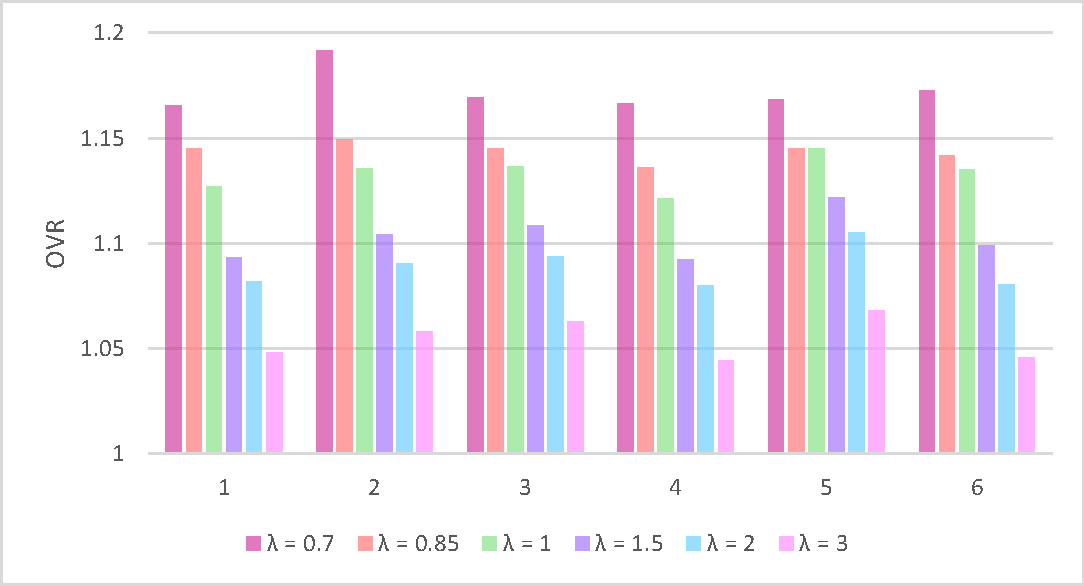
\includegraphics[width = \columnwidth]{plots/alpha.pdf}%
\caption{Adjusting $\lambda$ provides a tradeoff between vertex caching and overdraw, as shown here for the six animations of the Ganfaul model.}
\label{fig:alpha}
\end{figure}

\begin{figure}[t]
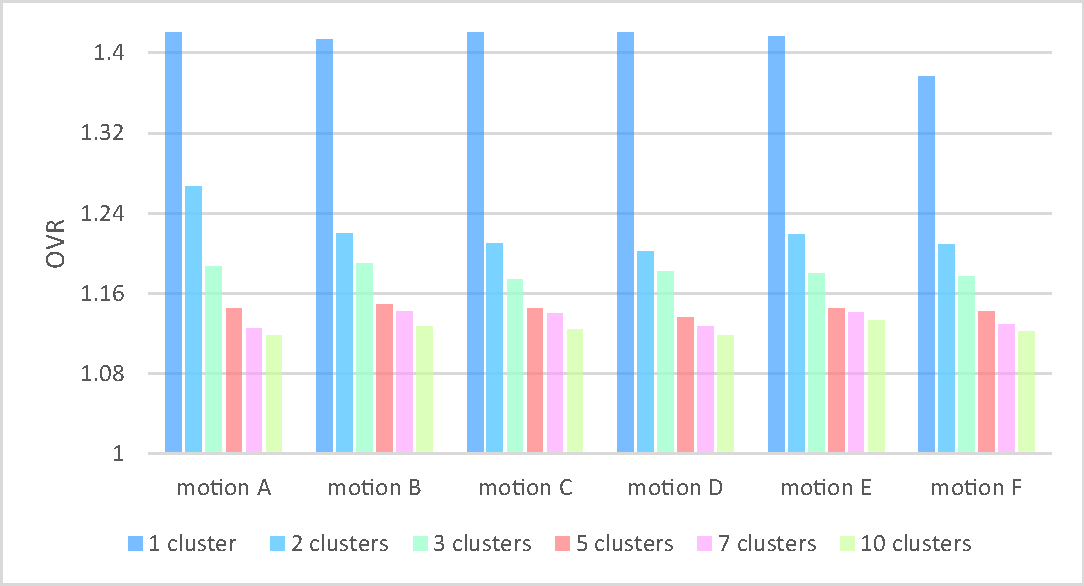
\includegraphics[width=\columnwidth]{plots/GanfaulClusters.pdf}
\caption{The number of clusters trades off memory (one index buffer per cluster) and overdraw, as shown here for the six animations of the Ganfaul model.}
\label{fig:clusters}
\end{figure}

\section{Results}
\label{sec:results}

In this section, we present results of our approach.
Our results use four models undergoing a set of six complex animations
that have between 30 and 70 keyframes.  These are representative of animated characters often found in games
and other real-time applications. Refer to the supplemental video for a demonstration of these animations.
Table~\ref{tab:preproc} shows preprocessing times for creating index buffers for each animation (labeled {\em A-F}), as well as
for a {\em joint} set of buffers that is optimized for all animations. Note that we did not heavily optimize
the preprocessing computation for speed, since this is done offline and only once after modeling. We focused on reducing overdraw for higher runtime performance
on pixel bound scenes.

\ignore{All experiments were conducted
on an Intel\textsuperscript{\textregistered}
Xeon\textsuperscript{\textregistered} 2.27GHz E5520 
CPU with 12GB of RAM and an AMD
Radeon HD 6970 GPU.}

\paragraph{Choice of $\boldsymbol\lambda$} As mentioned earlier, rendering time has been shown to be
directly proportional to ACMR for vertex-bound scenes, and OVR for pixel-bound
scenes~\citep{Sander07}. The algorithm trades off these objectives by controlling the
desired ACMR through the $\lambda$ parameter. Figure~\ref{fig:alpha} shows how the overdraw ratio is affected by the choice
of $\lambda$. We have found that setting $\lambda$ in the range of $0.75-0.95$ provides a
good balance between ACMR and OVR objectives for our animated scenes. For the remaining results in this paper, we use $\lambda=0.85$.
In addition, we also provide results for $\lambda=3$, which is the
extreme case where vertex cache performance is not taken into account and results
are solely optimized for reduced overdraw.

\paragraph{Choice of number of clusters} Figure~\ref{fig:clusters} shows results for different number of clusters for the Ganfaul model.
Increasing the number of clusters reduces overdraw at the expense of memory to store the additional index
buffers. We have found that using more than five clusters only yields modest ovedraw reduction for the models and animations that we tested. Thus,
for the remaining results in the paper, we use five clusters.

\paragraph{Overall results} Table~\ref{tab:stats} shows the statistics of each of our four models. Results are averaged over all keyframes and over a set of 300 random viewpoints within a radius three times that of the object's bounding sphere. The {\em original} results use a single index buffer that is optimized solely for reduced ACMR. It has a low memory footprint since it only requires one buffer, however it results in an order with high overdraw. The {\em tipsify} results use the state-of-the-art algorithm for static scenes described in ~\cite{Sander07} applied to {\em each individual frame}. It reduces overdraw significantly, but requires between 30-70 index buffers, depending on the animation, making its direct use impractical. Our {\em single} set of results uses five clusters for each single animation, thus requiring only five index buffers per animation and our cluster-based approach further reduces overdraw significantly for both $\lambda = 0.85$ and $\lambda = 3$. Our {\em joint} set of results optimize for the same five clusters for all frames in {\em all animations}. It therefore does slightly worse than the single animation results. As described earlier, the choice of $\lambda$ affects the resulting ACMR. With $\lambda = 0.85$, ACMR is kept under 0.9, while for $\lambda = 3$, the order is solely optimized for overdraw, thus ACMR is significantly sacrificed to achieve this additional reduction in overdraw. Figure~\ref{fig:results} further breaks down the results for each animation (labeled {\em motion A-F}). Note that the improvements of our algorithm are consistent over a variety of different character animations and brings the overdraw ratio very close to the optimal value of 1.

\paragraph{Rendering times} We conducted experiments to verify the dependency between OVR and rendering time~\citep{Sander07}. We used the Kachujin model with $\alpha=0.85$ in a heavily pixel bound scene. We noticed the improvement in rendering time closely matched the improvement in OVR ($\sim$18-20\%). With an inexpensive shader that simply outputs the color, the improvement was less significant ($\sim$10\%).

\begin{table*}
\newcolumntype{Y}{>{\centering\arraybackslash}X}
\newcommand{\ce}[1]{\multicolumn{1}{c}{#1}}
\caption{Average cache miss ratio (ACMR) and overdraw ratio (OVR) results for several character animations. We contrast our method with a triangle order that only considers vertex caching (original), and with the approach for static meshes of \cite{Sander07}, which applies the algorithm to each frame independently, resulting in 30-70 index buffers per animation (tipsify). We present our results using a separate set of five index buffers per motion (single) and with a joint set of five index buffers for all motions combined (joint).}
\label{tab:stats}
\begin{center}
\setlength{\tabcolsep}{3.2pt}
\footnotesize
%\small
\begin{tabularx}{\textwidth}{lr *{14}{Y}}
\toprule
\multirow{2}*{Model} &
\multirow{2}*{\# tris} &
\multicolumn{2}{c}{Original} &
\multicolumn{2}{c}{Tipsify ($\lambda=0.85$)} &
\multicolumn{2}{c}{Tipsify ($\lambda=3$)} &
\multicolumn{2}{c}{Single ($\lambda=0.85$)} &
\multicolumn{2}{c}{Single ($\lambda=3$)} &
\multicolumn{2}{c}{Joint ($\lambda=0.85$)} &
\multicolumn{2}{c}{Joint ($\lambda=3$)} \\
\cmidrule(l{2pt}r{2pt}){3-4}
\cmidrule(l{2pt}r{2pt}){5-6}
\cmidrule(l{2pt}r{2pt}){7-8}
\cmidrule(l{2pt}r{2pt}){9-10}
\cmidrule(l{2pt}r{2pt}){11-12}
\cmidrule(l{2pt}r{2pt}){13-14}
\cmidrule(l{2pt}r{2pt}){15-16}
& & {\emph{ACMR}} & {\emph{OVR}} & {\emph{ACMR}} & {\emph{OVR}} & {\emph{ACMR}} & {\emph{OVR}} & {\emph{ACMR}} & {\emph{OVR}} & {\emph{ACMR}} & \ce{\emph{OVR}} & {\emph{ACMR}} & \ce{\emph{OVR}} & {\emph{ACMR}} & \ce{\emph{OVR}}\\
\midrule
%Ganfaul & 13,801 & 0.676 & 1.351 & 0.869 & 1.296 & 2.939 & 1.214 & 0.860 & 1.139 & 2.715 & 1.054\\
%Kachujin & 12,610 & 0.645 & 1.308 & 0.903 & 1.178 & 2.896 & 1.120 & 0.891 & 1.076 & 2.619 & 1.024\\
%Maw & 13,908 & 0.619 & 1.395 & 0.879 & 1.255 & 2.918 & 1.165 & 0.860 & 1.097 &  2.694& 1.036\\
%Nightshade & 12,996 & 0.656 & 1.309 & 0.862 & 1.178 & 2.930 & 1.114 & 0.854 & 1.067 & 2.640 & 1.022\\
Ganfaul & 13,801 & 0.676 & 1.355 & 0.869 & 1.298 & 2.939 & 1.213 & 0.862 & 1.144 & 2.715 & 1.055 & 0.860 & 1.144 & 2.684 & 1.064\\
Kachujin & 12,610 & 0.645 & 1.310 & 0.903 & 1.172 & 2.896 & 1.122 & 0.891 & 1.068 & 2.617 & 1.027 & 0.887 & 1.102 & 2.570 & 1.030 \\
Maw & 13,908 & 0.619 & 1.380 & 0.879 & 1.253 & 2.918 & 1.166 & 0.860 & 1.101 &  2.696 & 1.038 & 0.859 & 1.109 & 2.675 & 1.044 \\
Nightshade & 12,996 & 0.656 & 1.302 & 0.862 & 1.172 & 2.930 & 1.112 & 0.854 & 1.068 & 2.643 & 1.024 & 0.854 & 1.071 & 2.612 & 1.027 \\
\bottomrule
\end{tabularx}
\bigskip
\end{center}
\vspace*{-1.5ex}
\end{table*}

\begin{figure*}[t]
\centering
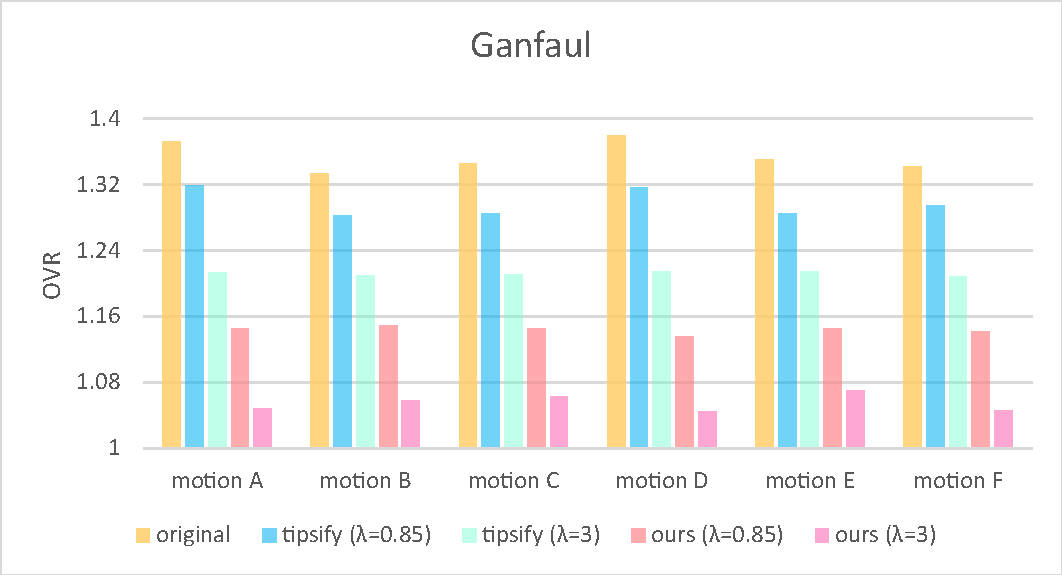
\includegraphics[width=.49\textwidth]{plots/GanfaulRatio.pdf}
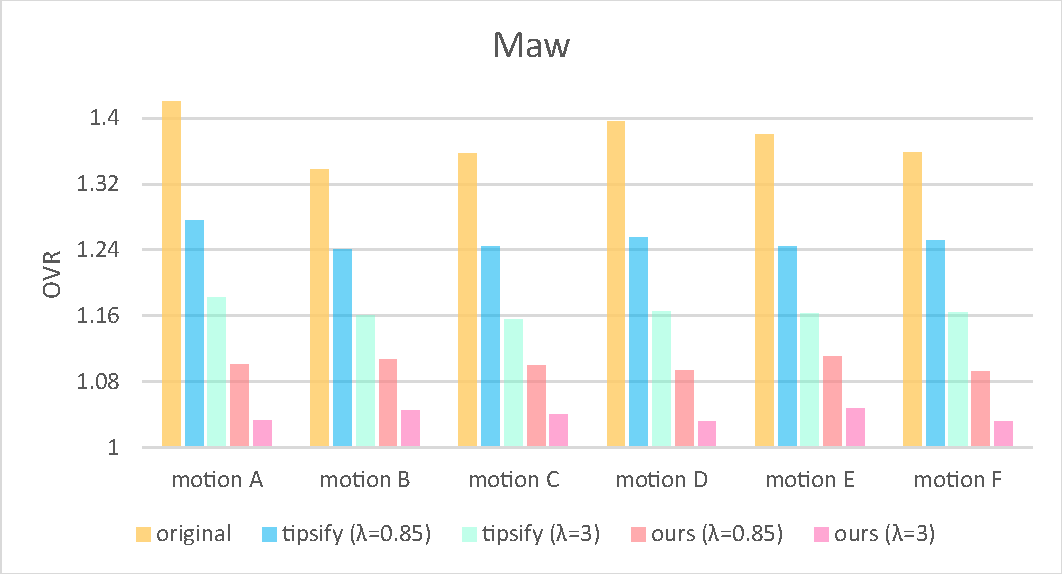
\includegraphics[width=.49\textwidth]{plots/MawRatio.pdf}
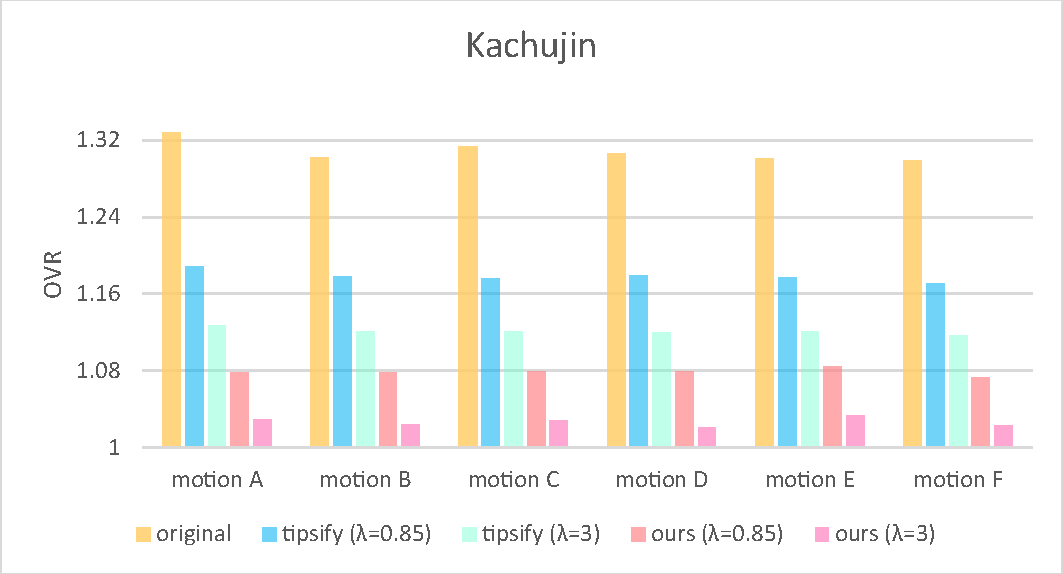
\includegraphics[width=.49\textwidth]{plots/KachujinRatio.pdf}
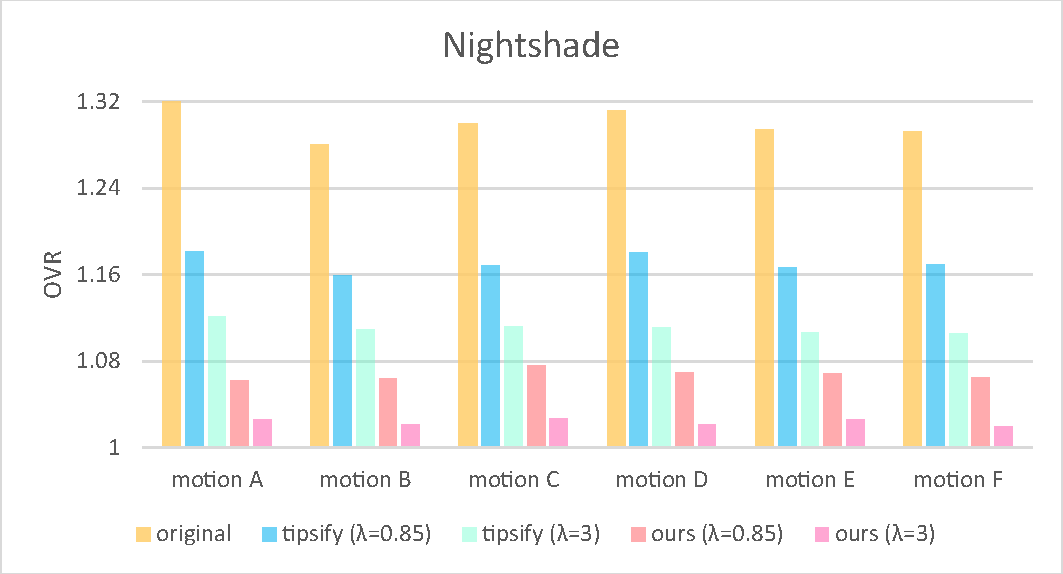
\includegraphics[width=.49\textwidth]{plots/NightshadeRatio.pdf}
\caption{Average overdraw ratio for different animations of the four models from Table~\ref{tab:stats}.}
\label{fig:results}
\end{figure*}

\ignore{??
Patch position is area-weighted
Normalize center position of frame to avoid giving higher distance weights to some frames in the presence of motion

??Using multiple buffers is what makes our overdraw better. tipsify restricted to one per frame
}








\section{Conclusion}

We introduced a new algorithm to efficiently reorder triangles
of animated models in order to reduce overdraw. To our knowledge,
this is the first technique that generates such optimized triangle orders for
animations. By using a small number of index buffers, the proposed 
approach produces triangle orders that have significantly
 lower overdraw even when compared 
to techniques that are optimized for static meshes. We presented results
that balance between vertex cache and overdraw performance
as well as results that are solely optimized for reduced overdraw. The approach
is very general and widely applicable to arbitrary animations
in a variety of real-time rendering applications.


\section*{Acknowledgments}

This work was partly supported by Hong Kong GRF grants
\#619509 and \#618513. The models used are from Mixamo.

%\bibliographystyle{acmsiggraph}
\bibliography{animorder}
\end{document}
